\documentclass[]{IEEEibm}

\usepackage[colorlinks,urlcolor=blue,linkcolor=blue,citecolor=blue]{hyperref}

\usepackage{upmath}

\jvol{XX}
\jnum{XX}
\paper{8}
\jmonth{February}
\pubyear{2020}
\newtheorem{theorem}{Theorem}
\newtheorem{lemma}{Lemma}

\setcounter{secnumdepth}{0}

\begin{document}

\title{Title: The Piracy World of the STB Providers}

\author{Author : M. J.}

\markboth{Author : Mohamed JAAFAR}{The Piracy World of the STB}

\begin{abstract}
This Document is related to the piracy architecture used in the market to hide the big parallel streaming network used for several clients not wanting to pay the subscriptions for TV operators. 
\end{abstract}

\maketitle


% too much jokes no good dude lol 
\section{Introduction : Content and STB market losses from Piracy}

The STB market today has grow at a point that the way of delivering the streams is not only on satellite, the cable and TNT. Operators nowaday use the triple play offer to feed the market of TV and sometimes the opposite from telephony and mobile market in this case we talk about the qudriplay offers. The TV market offers vary from free To View TV to susbcription TV ones. The case of Subscriptions via TV operators has been enhanced by to many new improvements like nPVR in the IPTV streaming world nVoD for the TNT or Satellite for example. So, In this market the industruals like too many of them that had already targeted the Business to Business Brand market had grow the market of the Business to Custumers called the Retail. In the Pay TV world there are two was of entitlements : Subscription and entitlements and even license in case of VoD for example or nPVR.

The encryption solutions varied from card for cable TNT and Satellite to cardless for IPTV using license like DRMs for VoD content like on youtube for example. For the Satellite solutions specially manufacturers use the common card module from years ago and some maybe would use the internet right solution that would be better way to fit the cardless of the IPTV solution to reduce the product cost like IRDETO Advanced Security cardless. `We are not here to make ads for IRDETO - kudelski But, It's one of the best ways to reduce piracy and costs`.

The Free TV market holded so many manufacturers using proprietary softwares and open source software. The most interessing solutions are the opensource ones. Some communities added good ideas to provide opensource softwares and interfaces like Enigma and Blackout on Vu and Dreambox and so many others. The community added many new features and solutions sometimes lacking on the propriety softwares which is nice to have like VFD feature on VuPlus and the sourcecode itself if you want to add your own packages on \href {https://github.com/OpenVuPlus/dvbapp}{Vu Plus opensource repository}. Some other solution are in IPTV with no operators devices like Sling or Hulu as pay TV or \href {https://pluto.tv}{Pluto TV} the new IPTV package with good content. using android or any couch potatoe devices no the cleaner. 


Even with the growth of the offers and market some would choose the freeTV. But, still want to get premium content. In this case the parallel world of the Piracy comes to make you watch TVshow and BoxOffice movies for less prices. Our subject in here How to detect the Piracy network of the illigal pay tv mesh and how to deal with it if we can.

\section{Piracy Target STBs and Piracy software structure}
The Parallel market is so big that you can find too many receivers on the internet using the application \href {https://openpli.org/}{OpenPLI} for web interface called OpenWebIF based on the http server called  \href{https://twistedmatrix.com}{TwistedWeb} to export the \href {https://www.enigma2.net/}{Enigma2} application services. 

\begin{figure}
\centerline{ 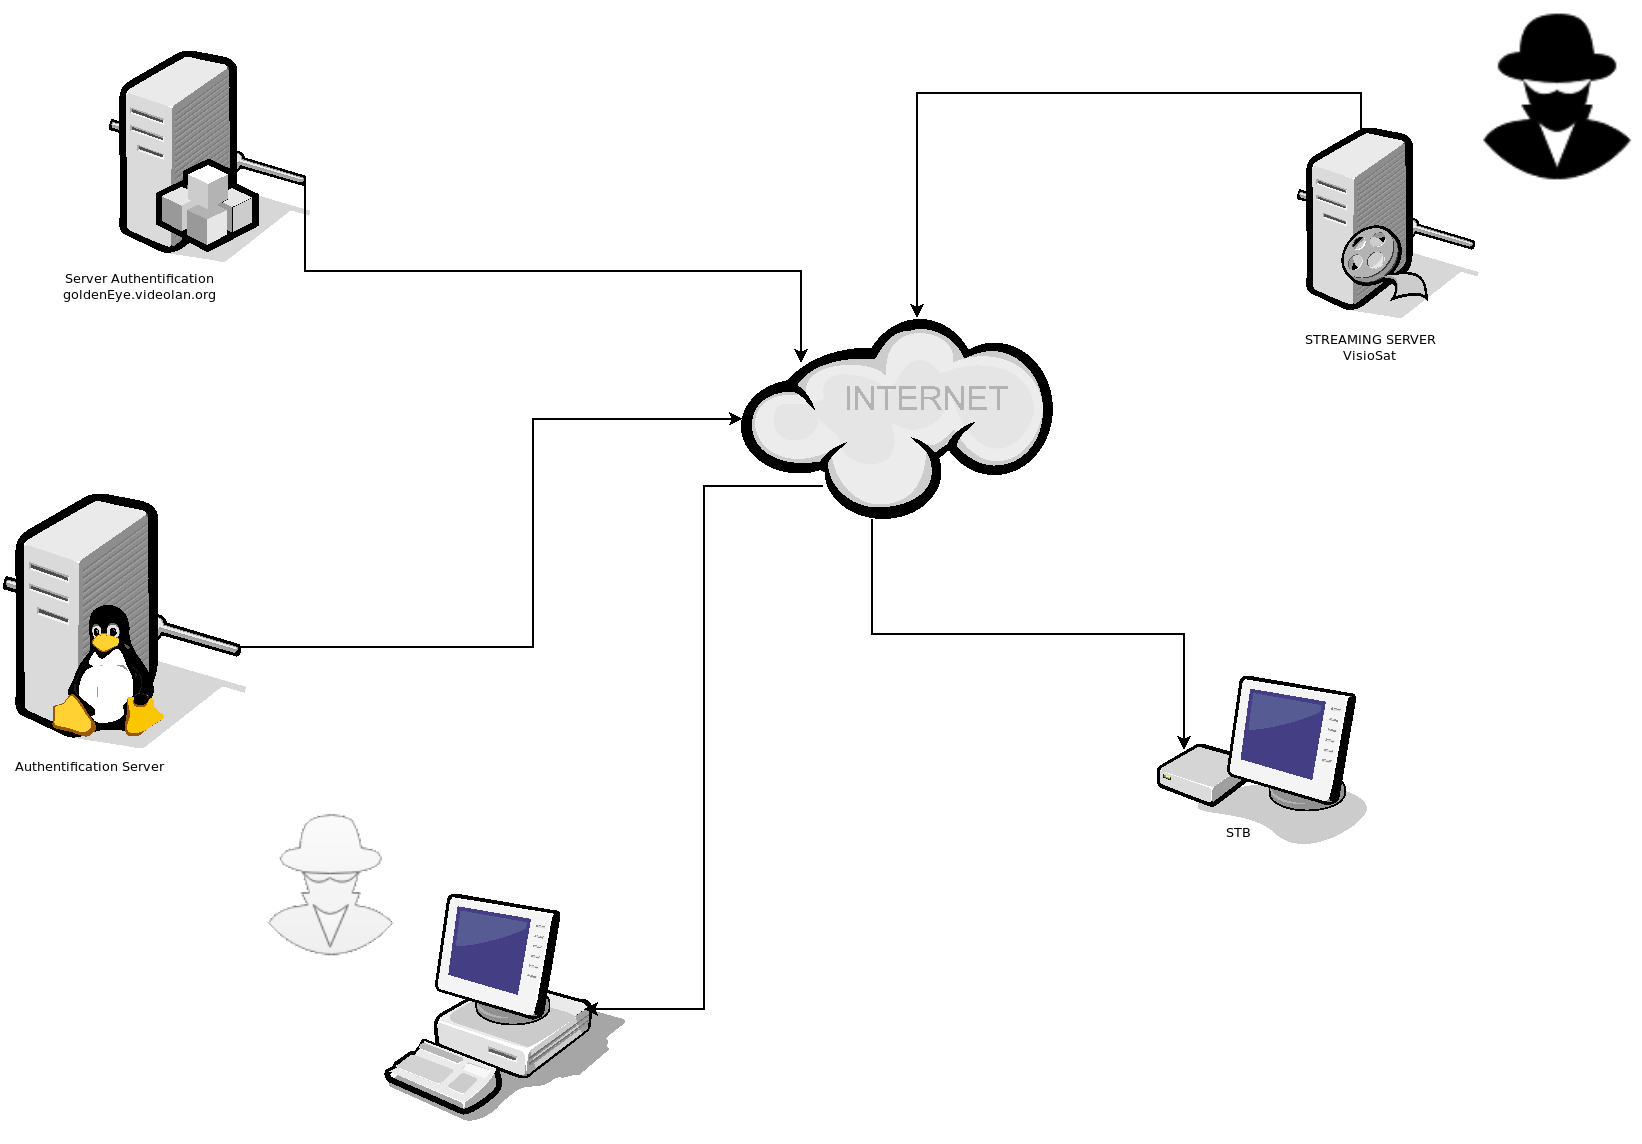
\includegraphics[width=18.5pc]{PiracyStreamingArchitecture.png}}
 % PiracyStreamingArchitecture.png: 1642x1144 px, 72dpi, 57.93x40.36 cm, bb=0 0 1642 1144
 \caption{Parallel stb streaming network}
\end{figure}



\section{Piracy Platform Architecture}


\section{Conclusion}

The manuscript should include a conclusion. In this section, summarize what was described in your paper. Future directions may also be included in this section. Authors are strongly encouraged not to reference multiple figures or tables in the conclusion; these should be referenced in the body of the paper.

\section{Acknowledgment}

This work was supported in part by a grant from family with their encouragement for good things the best values to support.


\begin{thebibliography}{1}

\bibitem{AA1}
G.M. Amdahl, G.A. Blaauw, and F.P. Brooks, ``Architecture\break of the IBM System/360,'' {\it IBM J. Res. \& Dev}., vol. 8, no. 2,\break pp. 87--101, 1964. (journal)

\bibitem{BB1}
IBM Corporation, IBM Knowledge Center - IBM Secure Service Container (Secure Service Container). [Online]. Available: {https://www.ibm.com/support/knowledgecenter/en/HW11R/\break com.ibm.hwmca.kc\_se.doc/introductiontotheconsole/wn2131zaci.html} (URL)

\end{thebibliography}


\begin{IEEEbiography}{Wireshark.}\textit{Wireshark is the world\'s foremost network protocol analyzer}. It lets you see what\'s happening on your network at a microscopic level. It is the de facto (and often de jure) standard across many industries and educational institutions. Wireshark development thrives thanks to the contributions of networking experts across the globe. It is the continuation of a project that started in 1998.
\end{IEEEbiography}

\begin{IEEEbiography}{Metasploit.}\textit{The Metasploit Framework is a Ruby-based, modular penetration testing platform that enables you to write, test, and execute exploit code}. The Metasploit Framework contains a suite of tools that you can use to test security vulnerabilities, enumerate networks, execute attacks, and evade detection. At its core, the Metasploit Framework is a collection of commonly used tools that provide a complete environment for penetration testing and exploit development.
\end{IEEEbiography}

\begin{IEEEbiography}{Python.}\textit{ Python is an interpreted, object-oriented, high-level programming language with dynamic semantics}. Its high-level built in data structures, combined with dynamic typing and dynamic binding, make it very attractive for Rapid Application Development, as well as for use as a scripting or glue language to connect existing components together. Python's simple, easy to learn syntax emphasizes readability and therefore reduces the cost of program maintenance. Python supports modules and packages, which encourages program modularity and code reuse. The Python interpreter and the extensive standard library are available in source or binary form without charge for all major platforms, and can be freely distributed.

Often, programmers fall in love with Python because of the increased productivity it provides. Since there is no compilation step, the edit-test-debug cycle is incredibly fast. Debugging Python programs is easy: a bug or bad input will never cause a segmentation fault. Instead, when the interpreter discovers an error, it raises an exception. When the program doesn't catch the exception, the interpreter prints a stack trace. A source level debugger allows inspection of local and global variables, evaluation of arbitrary expressions, setting breakpoints, stepping through the code a line at a time, and so on. The debugger is written in Python itself, testifying to Python's introspective power. On the other hand, often the quickest way to debug a program is to add a few print statements to the source: the fast edit-test-debug cycle makes this simple approach very effective. 
 
\end{IEEEbiography}


\begin{IEEEbiography}{Second B. Author Jr.}\textit{ABC Corporation, Böblingen, Germany (sbauthor@abc.com)}. Ms. Author’s biography appears here.
\end{IEEEbiography}

\begin{IEEEbiography}{Third C. Author III}\textit{DEF Corporation, Tokyo, Japan (tcauthor@def.com)}. Dr. Author’s biography appears here.
\end{IEEEbiography}

\end{document}
